\documentclass{article}

\usepackage[utf8]{inputenc}
\usepackage{tikz}
\usepackage{amsmath}
\usepackage{mathtools}
\usepackage{amsfonts}
\usepackage{amssymb}
\usepackage{sectsty}
\usepackage{xcolor}
\usepackage[paperwidth=180mm, paperheight=290mm, left=10mm, top=10mm, bottom=10mm, right=10mm, margin=10mm]{geometry}
\usepackage{ragged2e}
\usepackage{listings}

\definecolor{def}{RGB}{255, 173, 97}
\definecolor{tit}{RGB}{217, 84, 80}
\definecolor{emp}{RGB}{150, 206, 180}
\definecolor{acc}{RGB}{255, 238, 173}
\definecolor{txt}{RGB}{249, 232, 232}
\definecolor{back}{RGB}{22, 22, 22}

\sectionfont{\color{tit}\fontsize{20.74}{35}\ttfamily}
\subsectionfont{\color{tit}\fontsize{17.28}{17.28}\ttfamily}

\DeclareFontFamily{\encodingdefault}{\ttdefault}{%
  \hyphenchar\font=\defaulthyphenchar
  \fontdimen2\font=0.33333em
  \fontdimen3\font=0.16667em
  \fontdimen4\font=0.11111em
  \fontdimen7\font=0.11111em
}

\newcommand{\R}{\mathbb{R}}
\newcommand{\N}{\mathbb{N}}
\newcommand{\Q}{\mathbb{Q}}
\newcommand{\Z}{\mathbb{Z}}
\newcommand{\C}{\mathbb{C}}
\newcommand{\cont}{\mathfrak{c}}

\geometry{a4paper, textwidth=155mm, textheight=267mm, left=15mm, top=15mm, right=15mm, marginparwidth=0mm}
\setlength\parindent{15pt}

\pagestyle{empty}

\begin{document}\pagecolor{back}\color{txt}\ttfamily
\section*{NIEPORZADKI}
    \begin{center}
        Nieporzadkiem na danym zbiorze nazywamy \color{def}permutacje jego elementow bez punktow stalych\color{txt}.\smallskip\\
        (\emph{bijekcja bez punktow stalych})
    \end{center}
    Jak przy losowaniu komu kupimy prezent na mikolajki - nie chcemy kupowac prezentu sobie samemu. Jak czesto sie zdarza, ze ktos wylosuje siebie samego?
    $$\color{acc}D_n=n!\;(1-\frac1{1!}+\frac1{2!}+...+(-1)^n\frac1{n!})$$
    \color{emp}DOWOD\color{txt}:\medskip\\
    Ze zbioru wszystkich permutacji $S_n$, ktory ma moc $n!$ odejmujemy zbiory, w ktorych $i$ zostaje na swoim miejscu:
    $$D_n=|S_n|-|Z(1)\cup Z(2)\cup...\cup Z(n)|$$
    Stosujemy zasade z poprzedniego wykladu:
    $$|Z(1)\cup Z(2)\cup...\cup Z(n)|=|Z(1)|+|Z(2)|+...+|Z(n)|-(|Z(1)\cap Z(2)|+|Z(1)\cap Z(3)|+...)+...$$
    Mamy $|Z(i)|=(n-1)!$, bo nie ruszamy jednego elementu, a reszta moze sie przemieszczac dowoli. Analogicznie $|Z(i)\cap Z(j)|=(z-2)!$. Pokolei rozpiszmy prawa strone rownania:
    $$Z(n)|=|Z(1)|+|Z(2)|+...+|Z(n)| = n\cdot(n-1)!$$
    bo mamy $n$ zbiorow, kazdy o mocy $(n-1)!$.
    $$|Z(1)\cap Z(2)|+|Z(1)\cap Z(3)|+...={n\choose2}(n-2)!$$
    czyli dwa zbiory mozemy wybrac na ${n\choose2}$ sposobow, a ich przekroj ma moc $(n-2)!$.\\
    Rozpiszmy rownanie:
    $$|Z(1)\cup Z(2)\cup...\cup Z(n)|=|Z(1)|+|Z(2)|+...+|Z(n)|-(|Z(1)\cap Z(2)|+|Z(1)\cap Z(3)|+...)+...=$$
    $$=n(n-1)!-{n\choose2}(n-2)!+{n\choose3}(n-3)!+...=n!(1-{1\over1!}+{1\over2!}-...)$$
    Z analizy matematycznej wiemy, ze
    $$1-{1\over1!}+{1\over2!}-...\approx{1\over e}$$
\subsection*{REKURENCJE}
    \begin{center}
        \emph{\color{emp}Ciag wyrazow rekurencyjnych to taki ciag, w ktorym $n$ wyraz \\wyliczamy w zaleznosci od poprzednich wyrazow.}
    \end{center}
    Przyblizanie pierwiastka z $a$:
    \begin{align*}
        a&>0\\x_0&=a\\
        x_n&={1\over2}(x_{n-1}+{a\over x_{n-1}})\\
        g&=\frac12(g+\frac{a}{g})=\sqrt{a}\bigskip
    \end{align*}
    \color{def}CIAG FIBONACCIEGO\color{txt}: Ile jest ciagow o wyrazach 1, 2, ktorych suma wynosi $n$?
    $$x_n=x_{n-1}+x_{n-2}$$
    $$x_1=1,\;x_2=2$$
    wynik to ilosc sposobow, na jakie mozemy wyliczyc $n$ uzywajac liczb naturalnych liczb 1 i 2.\medskip\\
    \color{emp}DOWOD:\color{txt}\medskip\\
    Mamy \color{acc}$k$ przegrodek\color{txt}, w ktore mozemy wstawiac 1 i 2 tak, zeby uzyskac $n$. Na koncu moze byc  1 albo 2. Jesli na koncu jest 1, to na poprzednich miejscach musialo byc $n-1$, a jesli 2, to na porpzednich musialo byc $n-2$. Poniewaz mozliwosci sa rozlaczne, to do pierwszego przypadu mamy \color{acc}$x_{n-1}$ mozliwosci dojscia, a do przypadku z 2 na kocu, mamy $x_{n-2}$ \color{txt}mozliwosci dojscia.\bigskip\\
    \color{def}NIEPORZADKI REKURENCYJNIE\color{txt}: dla $n\geq 3$
    $$\color{acc}D_n=(n-1)(D_{n-2}+D_{n-1})$$
    \color{emp}DOWOD\color{txt}:\medskip\\
    Podzielmy nieporzadki na zbiorze $\{1, ..., n\}$ na dwie klasy.\smallskip\par
        \color{tit}1. \color{txt}element $n$-ty przechodzi na $i<n$, ale $i$ przechodzi jednoczesnie na $n$.\par
        Jest $(n-1)\cdot D_{n-2}$ takich nieporzadkow, bo biore element $i$ na $n-1$ sposobow, usuwam $n$ i $i$, wiec na pozostalych musze utowrzyc nieporzadek.\par
        \color{tit}2. \color{txt}$n$ przechodzi na $i<n$, ale $i$ nie przechodzi na $n$, tylko na $j<n$. \par
        Jest $(n-1)D_{n-1}$ takich nieporzadkow. \color{tit}Wciskamy $n$ na jakies miejsce wsrod $n-1$ elementow \color{txt}- ile jest nieporzadkow na $n-1$ elementach.\smallskip\\
    Zliczamy obie klasy i dostajemy $D_n$.\bigskip\\
    \color{emp}PRZYKLAD\color{txt}: Na ile sposobow mozna polaczyc elementy zbioru mocy $2n$ w pary?\smallskip\\
    Wybieram pierwsza pare
    $${2n\choose 2},$$
    wybieram druga pare
    $${2n\choose2}\cdot{2n-2\choose2}$$
    i tak dalej
    $${2n\choose2}\cdot{2n-2\choose2}\cdot...{2\choose2}.$$
    Ale my nie numerujemy tych par, wiec musimy to podzielic na $n!$
    $${{2n\choose2}\cdot{2n-2\choose2}\cdot...{2\choose2}\over n!}.$$
    \color{acc}Rozwiazanie rekurencyjne:\color{txt}\smallskip\\
    Niech $x_n$ bedzie szukana liczba. Musimy napisac, jak sie ma $x_n$ do poprzednich wyrazow.\\
    Mamy $2n$ elementow, zaznaczamy element ostatni i dobieramy mu pare. Mozemy to zrobic na $2n-1$ sposobow, wiec
    $$x_n=(2n-1)x_{n-1}$$
    czyli jak sie to przeliczy otrzymujemy
    $$x_n=(2n-1)(2n-3)(2n-5)...\bigskip$$
    \color{def}WIEZE W HANOI\color{txt}\smallskip\\
    Mamy 3 prety: A, B i C. Na pierwszym precie jest $n$ malejacych krazkow, ktore chcemy przelozyc na drugi pret, ale mozemy tylko manipulowac pierwszym z gory i nie mozemy polozyc wiekszego krazka na mniejszy.\smallskip\\
    podejscie informatyczne - \color{tit}przekopiowac moj kod z WDI\color{txt}
\subsection*{UKLADY ROWNAN REKURENCYJNYCH}
    Ile jest ciagow dlugosci $n$ o wyrazach z $\{0,1,2\}$ takich, ze kazdy nastepny wyraz jest o 1 wiekszy lub o jeden mniejszy?
    Przedstawmy to jako \color{acc}pileczke odbijajaca sie miedzy 3 liniami\color{txt}:
    \begin{center}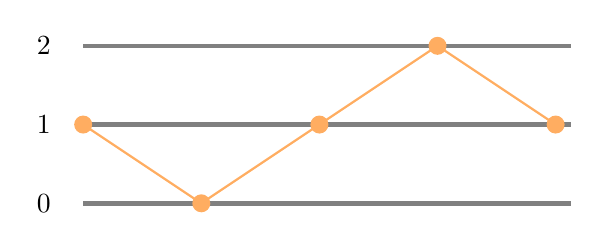
\begin{tikzpicture}
        \draw[gray, ultra thick] (0, 0)--(6.2,0);
        \draw[gray, ultra thick] (0, 1)--(6.2, 1);
        \draw[gray, ultra thick] (0, 2)--(6.2, 2);
        \draw[def, thick] (0,1)--(1.5,0);
        \draw[def, thick] (1.5, 0)--(3,1);
        \draw[def, thick](3,1)--(4.5,2);
        \draw[def, thick](4.5,2)--(6, 1);
        \filldraw[color=def, fill=def, thick] (0,1) circle (0.1);
        \filldraw[color=def, fill=def, thick] (1.5, 0) circle (0.1);
        \filldraw[color=def, fill=def, thick] (3, 1) circle (0.1);
        \filldraw[color=def, fill=def, thick] (4.5, 2) circle (0.1);
        \filldraw[color=def, fill=def, thick] (6,1) circle (0.1);
        \node(1) at (-0.5, 1) {1};
        \node(2) at (-0.5, 2) {2};
        \node(0) at (-0.5, 0) {0};
    \end{tikzpicture}\end{center}
    Niech $a_n$ bedzie iloscia szukana. \color{acc}Nie da sie tego zrobic od razu, wiec podzielmy liczbe $n$ na dwie czesci\color{txt}:\smallskip\par
        $a_n^1$ to liczba ciagow konczacych sie na 1\par
        $a_n^{0,2}$ to liczba ciagow konczacych sie na 0 lub 2.\medskip\\
    Ilosc pierwszej czesci: chcemy konczyc na 1, wiec musielismy byc w 0 lub 2. Dopisujemy do krotszego ciagu 1 i gotowe
    $$a_n^1=a_{n-1}^{0,2}.$$
    Ale mozemy popatrzec dwa miejsca w tym - bylismy w 1 i chcemy wrocic na 1. Moglismy zachaczyc o 0 lub o 2, wiec mamy dwie mozliwosci.
    $$a_n^1=2\cdot a_{n-2}^1$$
    Znamy pierwsze wyrazy:
    $$a_n^1=1,\quad a_2^1=2$$
    Mozemy znalezc wzor jawny:
    $$a_n^1=2^{[\frac{n}2]}$$
    I wzor ogolem:
    $$a_n=a_n^1+a_n^{0,2}=a_n^{[\frac{n}2]}+a_n^{[\frac{n+1}2]}$$
    \color{emp}PRZYKLAD\color{txt}: Na ile sposobow mozna zbudowac plotek o wymiarach 2 $\times$ $n$ majac do dyskozycji klepki 1 $\times$ 2?\\
    \begin{align*}
        x_0&=1\\
        x_1&=1\\
        x_2&=2\\
        x_n&=x_{n-1}+x_{n-2}
    \end{align*}
\end{document}